\section{Experimental Evidence}
\label{sec:experiments}

We test coupling, trained-activation uncertainty, and GPU execution separately.
\Cref{sec:experimental-validation} records arithmetic and implementation
checks, including an executable interval defect found and repaired.

\subsection{Coupling and Localized Uncertainty}
\label{sec:coupling-experiment}

Coupling accepts four more initial coordinates than the box certificate, but
the global value hull explains three of those gains
(\cref{tab:coupling-results,fig:coupling-ablation}). The exact-rational study
uses seed 962605, four retained ranks, four key spreads, narrow and broad value
channels, exact midpoint channels, and named geometry and attention witnesses.
All 53 cases, 149 initial coordinates, and sequential refinement stages are
retained in \artifact{results/certification/coupling.json}{coupling artifact}, including construction
and actual rational fallback costs.

If all values lie in one rounding cell, positivity of attention weights already
certifies the output. The remaining prescribed witness instead places keys
$-2,2$ with values $1-1/2560,1+1/2560$ in one rank-zero block and a singleton
key $-16$ with value $3$, at $q=1$. The outlier defeats the global hull, but its
small block mass lets the coupled test certify BF16 value $1$. An independent
direct rational exponential sum verifies the certificate. This witness
isolates the interaction between local value range and mass; it does not
estimate coverage on trained models.

\begin{figure*}[!t]
  \centering
  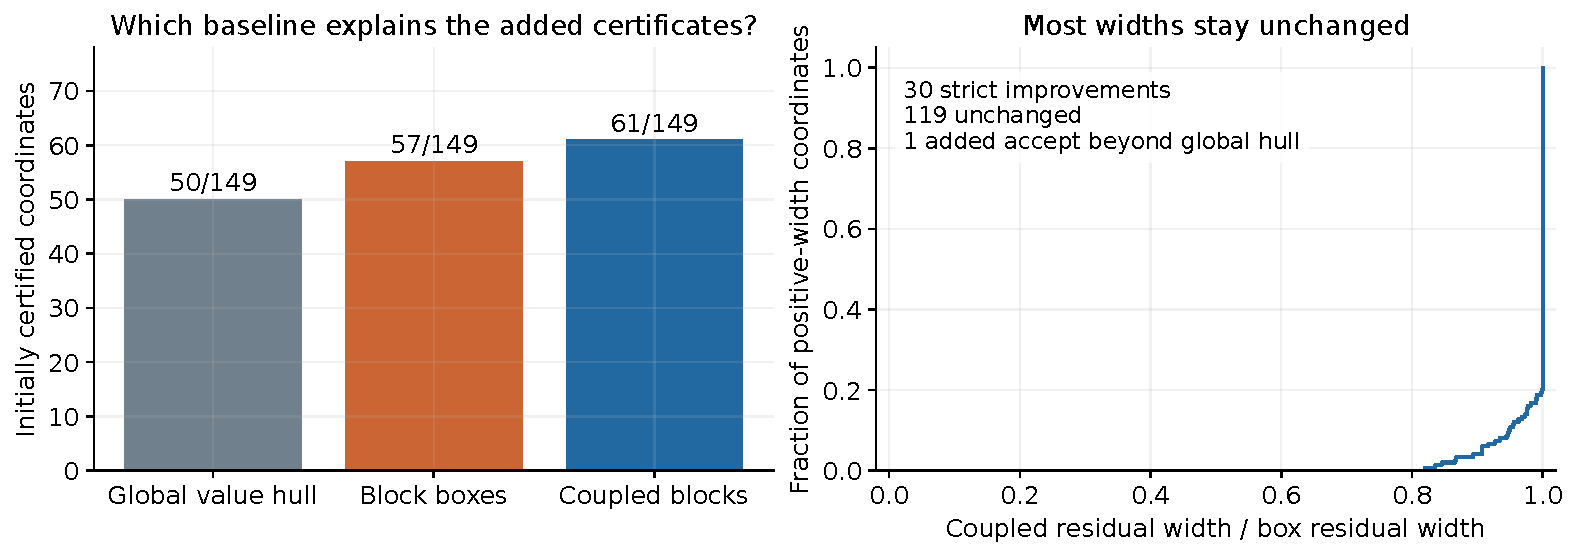
\includegraphics[width=\textwidth]{figures/coupling_ablation.pdf}
  \caption{Coupling acceptance and residual widths for all initial coordinates,
  retaining unchanged widths and refusals. The global-hull baseline explains
  most additional accepts.}
  \label{fig:coupling-ablation}
\end{figure*}

A numerical CPU experiment with $N=8192$, $d=16$, $h=8$, $B=16$, $Q=24$, and
one BLAS thread demonstrates when selective correction helps. The generator
provides favorable four-coordinate structure. Tight blocks pass all 24 queries
without correction; introducing one broad block makes every initial query fail,
but correcting that block evaluates attention weights and values for only
$1/16$ of the tokens. Broadening every block requires correcting every token
(\cref{fig:selective-refinement}). The correction-token counter excludes the
Python executor's full-source input validation and fingerprint passes, which
read K/V even without correction. CPU query times include these reads and
executed correction or fallback; construction is recorded separately.
Every complete Python path is slower than
dense NumPy: the experiment measures uncertainty localization, not GPU speed.


The GPU controls show why coordinate coverage alone is insufficient. Moderate
inputs pass 10,197 of 19,008 coordinates across repeated rank configurations,
but none of 297 complete outputs. A centered-value control passes 1,986 of
2,048 coordinates and only 6 of 32 outputs. Every coordinate must pass before
an output is accepted; any failure triggers the measured full-batch fallback.
\Cref{sec:localized-uncertainty} retains the control protocol and strict
midpoint refusals.

\subsection{Trained Post-RoPE Activations}
\label{sec:trained-activations}

Neither trained activation set produces a numerical coordinate or whole-output
pass. We capture post-RoPE Q/K/V from Qwen2.5-0.5B \citep{qwen25} on prose,
code, and arithmetic probes at prefix lengths 1,024 and 4,096. Rank eight
covers 24 layers and 14 query heads: 2,016 head instances and 129,024
coordinates. Full rank in layers 0, 12, and 23 adds 252 head instances.
\Cref{sec:trained-protocol} specifies the model revision and capture protocol.

At rank eight, $e^\epsilon-1$ amplifies centered-value uncertainty far beyond
cell margins. Full rank removes that term, but the broad retained radius makes
$\kappa(\rho)$ large (\cref{tab:trained-radii,fig:model-score-radii}). Median
maximum absolute candidate error is approximately $0.82$ at rank eight and
$0.50$ at full rank. Increasing rank therefore exchanges projection inflation
for Taylor inflation while leaving errors much larger than the narrowest
cells. \Cref{fig:model-error-budget} expresses the competing terms in output
units. Retained coordinates are a prefix of the actual transformed basis; no
learned basis, PCA fitting, or clustering was used. Other representations
remain untested, but must address within-block score variation, radius-bound
looseness, and value dependence together.

\begin{figure*}[!t]
  \centering
  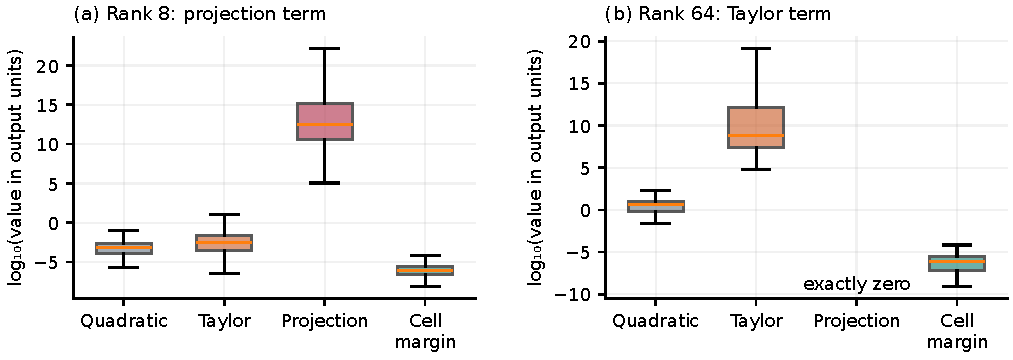
\includegraphics[width=\textwidth]{figures/model_error_budget.pdf}
  \caption{Maximum-channel omitted-quadratic, Taylor, and projection terms,
  divided by true shifted mass, compared with minimum-channel cell margins.
  These explain scales rather than additively decompose output error: mass
  uncertainty also contributes. JSON artifacts retain outliers beyond whiskers.}
  \label{fig:model-error-budget}
\end{figure*}

\subsection{GH200 Performance and Complete Costs}
\label{sec:gh200-measurements}

We measure 57 synthetic and nine trained prose trace/rank configurations on
one NVIDIA GH200. The forced PyTorch fused FlashAttention SDPA baseline
\citep{flashattention} matches BF16 inputs, scale, visible keys, and zero
dropout. Seven samples of 20 invocations provide CUDA-event and host-wall
times. Complete eager timings include screening, device decision reduction,
CPU synchronization, and output cast or actual full-batch fallback; resident
measurements exclude separately recorded setup. \Cref{sec:gh200-protocol}
gives the environment, batch semantics, and sampling details;
\cref{fig:gh200-latency} reports resident and complete-path latency.

Parallel block reduction improves the long-context, single-query resident
kernel, while small cases retain adverse results
(\cref{tab:gh200-ablation,fig:gh200-kernel-ablation}). Originally each output
coordinate occupies one thread looping serially over blocks; one query thus
exposes only 64 threads. Sharing repeated scalar arithmetic barely helps.
Assigning a CTA per coordinate exposes block parallelism, reducing the isolated
reduction from \SI{99.38}{\micro\second} to \SI{6.65}{\micro\second} at
$N=32768,Q=1$. With more queries or fewer blocks, additional CTAs and
synchronization provide less benefit and can hurt. Isolated phase measurements
diagnose this bottleneck; their sum does not replace measured complete latency
(\cref{fig:gh200-cost-breakdown}).

\begin{figure*}[!t]
  \centering
  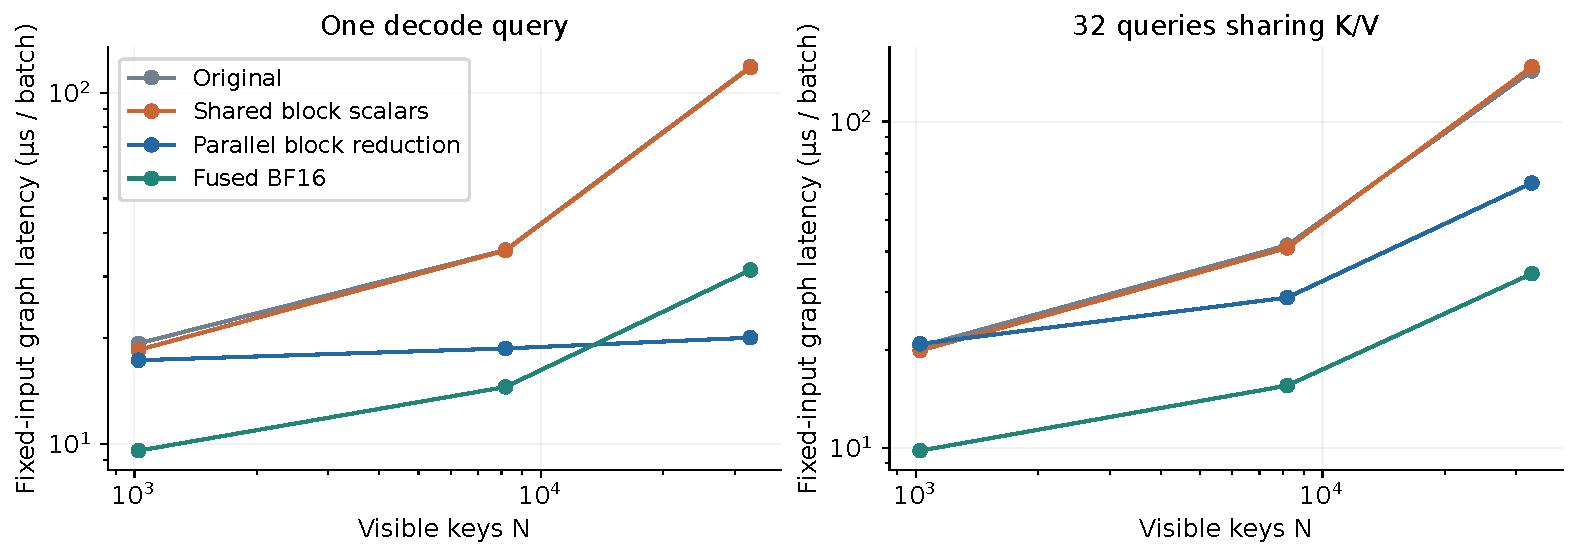
\includegraphics[width=\textwidth]{figures/gh200_kernel_ablation.pdf}
  \caption{Three CUDA implementations under matched graph replay. Sharing
  scalar work leaves serial block reduction dominant; parallelizing blocks
  helps long-context single-query inputs, with synchronization costs at small
  $N$.}
  \label{fig:gh200-kernel-ablation}
\end{figure*}

Even the favorable $N=32768,Q=1,r=4$ case loses end to end. Its resident
parallel screen takes \SI{20.09}{\micro\second} under fixed-input graph replay
versus dense attention's \SI{31.30}{\micro\second}; the complete eager path
takes \SI{83.11}{\micro\second} versus \SI{35.62}{\micro\second}, plus about
\SI{51.50}{\milli\second} of reusable summary/workspace setup. Every measured
complete path is slower than dense, so no finite reuse count repays setup
under these costs. \Cref{sec:gh200-costs} retains the footprint exclusions,
phase measurements, and amortization results.

\begin{samepage}
Across all 66 configurations, accepted numerical coordinates have zero observed
BF16 mismatches against binary64 attention but 1,691 against the fused BF16
baseline. Repeated configurations make these aggregate counts dependent.
Real-attention rounding and fused intermediate arithmetic are different
targets; the binary64 comparison is itself numerical, and the summary path is
not outward interval metadata for the directed checker.
\par
\end{samepage}


\begin{samepage}
A second run at committed implementation \texttt{d2c3668} reproduces all
66 cases with unchanged coverage and mismatch counts. Parallel-screen graph
medians change by $-1.08\%$ to $+1.42\%$, with median ratio $1.002$; every
complete path remains slower than dense. Figures and tables retain the first
sweep. \Cref{sec:gh200-reproduction} provides provenance, host-wall variation,
and the retained failed parity checks.
\par
\end{samepage}
